\subsubsection{Askoll eS1}
\label{apartado_moto_electrica}
\paragraph{Descripción general}
%%La motocicleta eléctrica Askoll eS1 es un scooter eléctrico de la empresa pionera en innovación de movilidad eléctrica Askoll de Italia. El scooter de la serie eS es ganador de muchos premios, incluido el Green Prix 2015.El eS1 está equipado con un motor eléctrico de 1.500 vatios con un par de 100 Nm, tiene una velocidad máxima de 45 km / h. El scooter cuenta con una batería de litio extraíble de 2,1 kWh para un alcance de 100 km y La batería se puede cargar en 6 horas.
Estudiando las consideraciones descritas en el \refanexo{anexo_scooter_electrico}, se ha escogido de entre todos los modelos mostrados el Askoll eS1 en la \autoref{fig:Askoll eS1}. 

\begin{figure}[h]
    \centering
    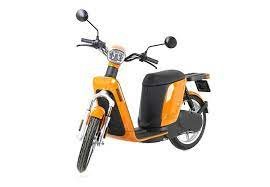
\includegraphics[scale = 0.8]{archivos/askoll es1.jpg}
    \caption{Askoll eS1.}
    \label{fig:Askoll eS1}
\end{figure}

Los motivos para elegir este modelo están basados en su gran autonomía frente a las demás opciones y un tiempo de carga bajo, lo que hace que sea la única opción realista de entre las eléctricas.

El scooter de la serie eS es ganador de muchos premios, incluido el Green Prix 2015. Está equipado con un motor eléctrico de 1.500 \glssymbol{vatios} con un par de 100 \glssymbol{par} y cuenta con una velocidad máxima de 45 \glssymbol{velocidad}. El scooter cuenta con una batería de litio extraíble de 2,1 \glssymbol{kilovatiohora} para un alcance de 100 \glssymbol{km} y la batería se puede cargar en 6 horas.

Cuenta con una autonomía de 100 \glssymbol{km} en ciudad, iluminación \gls{led}, suspensión hidráulica para una mayor estabilidad y frenos de disco para una mayor seguridad. Cuenta con neumáticos de 16 pulgadas para hacerlo más estable frente a las caídas. Un peso de tan solo 72 \glssymbol{kg} la hace muy ligera y manejable en todo tipo de situaciones.

% \paragraph{Estudio del reparto.}
%  %Escoger modelo
\paragraph{Mantenimiento y robustez}
%%Se trata de un modelo muy robusto ya que está concebido para realizar largas jornadas de trabajo. En cuanto al mantenimiento, como cualquier otra motocicleta eléctrica necesita el mantenimiento especificado en el "ANEXO X"(tabla con costes de mantenimiento).
Al ser un modelo eléctrico necesita menos mantenimiento que uno de gasolina, ya que no es necesario el cambio de aceite ni de transmisión. El modelo está construido en materiales de calidad para una mayor robustez.

Una motocicleta eléctrica necesita mantenimiento en sus frenos y ruedas, así como revisiones periódicas. Esto se estudia en el \refanexo{anexo_scooter_electrico}, obteniéndose un importe anual de mantenimiento de 126 \glssymbol{euro}.

\paragraph{Viabilidad económica}
%%El coste del primer año de esta motocicleta es de 3.348,94€ y de 663,94€ los años sucesivos  según lo calculado en el "ANEXO X".

%%Observando los resultados en \refanexo{anexo_scooter_electrico} y \autoref{consideraciones_preliminares_seguro} en los que se estudian detalladamente todos los costes que conlleva esta motocicleta se llega a un resultado final de que el coste que implica es de 2.685,00\glssymbol{euro} de inversión inicial para la compra de la motocicleta y de 753,44\glssymbol{euro} anuales en gastos.

Para ver si es factible el gasto hay que observar el gasto fijo que supone la adquisición del equipo al completo, y posteriormente el gasto anual entre mantenimiento, seguros y recargas. 

Todos los cálculos y estimaciones referentes a la viabilidad económica se pueden encontrar en la \autoref{tab:Estudio presupuestos modelo Askoll eS1}, \refanexo{sub_anexo_calculos_motocicleta_eléctrica}, donde se muestran los presupuestos para ambos modelos de reparto analizados en el estudio del reparto.

En el primer año, se han de tener en consideración el precio de mercado por unidad de las motocicletas eléctricas y el número total que se van a comprar, pues el impuesto de matriculación unitario es de 27,85 \glssymbol{euro}. Además de esto, hay que añadir como gasto fijo inicial la adquisición del equipamiento, los cuales se enumeran en la \autoref{consideraciones_preliminares}, considerando en cada caso el número de personal, o vehículos simultáneos en carretera.

Para los gastos anuales se debe comenzar con el coste de recarga del vehículo y el impuesto de circulación de 8,55 \glssymbol{euro}. Teniendo el precio de la luz, obtenido en el \refanexo{anexo_precio_taller_combustible} y el número de recargas semanales totales, junto con la capacidad de una batería, se obtiene el gasto semanal y anual relacionado con la recarga.

Los gastos relacionados con reparaciones o mantenimiento se han fijado en el \refanexo{anexo_scooter_electrico}, por lo que se asume un gasto mensual a cada uno. 

El coste por seguro fijado es de 265 \gls{euro}, lo cual se multiplicará directamente por el número de vehículos en posesión de manera mensual.

Teniendo todas las consideraciones anteriores descritas, se concluye finalmente el presupuesto necesario en el primer año y posteriores, recogidos en la \autoref{tab:Estudio presupuestos modelo Askoll eS1}, siendo:

\begin{itemize}
    \item Presupuesto para el primer año del modelo de estudio 1 - 30.475,64 \gls{euro}
    \item Presupuesto anual del modelo de estudio 1 - 5.107,09 \gls{euro}
    \item Presupuesto para el primer año del modelo de estudio 2 - 23.977,50 \gls{euro}
    \item Presupuesto anual del modelo de estudio 2 - 4.034,65 \gls{euro}
\end{itemize}

\paragraph{Conclusiones modelo.}
%%Es un modelo válido para la tarea debido a sus características y el bajo coste de mantenimiento.

Analizando los datos anteriores se concluye que dicha motocicleta es una opción con una gran autonomía, desempeño en su tarea y la opción más viable para cubrir largas distancias con pocas interrupciones. Todo esto teniendo en cuenta que tendrá que parar a recargarse cada 100 \glssymbol{km} para poder seguir con su labor de reparto.

De las opciones que se plantean es el vehículo eléctrico que alcanza la mayor velocidad y cuenta con la mayor autonomía de ellos, por lo que puede realizar un mayor número de repartos, necesitando por ello menos cantidad de ellas. Dada su clasificación dentro de los vehículos, no puede circular por autovías y autopistas en caso de que sea necesario, siendo este un factor a tener en cuenta para repartos.

Al ser un modelo de eléctrico no conlleva una contaminación, tanto medioambiental como en términos de ruido. A diferencia de las opciones de gasolina, la energía es más barata.